\documentclass{../llncs_template_final/llncs} 
\pagestyle{plain}
\usepackage[utf8]{inputenc}
\usepackage{polski}
\usepackage[polish]{babel}
\usepackage{makeidx}
\usepackage{algorithm}
\usepackage{algpseudocode}
%\usepackage{hyperref} % powoduje buga w LLNCS i nie możemy go użyć :(
\usepackage{graphicx}
\graphicspath{ {wykresy/} }
\begin{document}

\title{Teoria algorytmów i obliczeń -- Projekt -- Etap 3}
\author{Błażej Bobko, Jakub Gocławski, Patryk Kujawski, Radosław Kutkowski}
\institute{Wydział Matematyki i Nauk Informacyjnych, Politechnika Warszawska}
\maketitle 


\section{Opis zadania}

Zadanie polega na znalezieniu deterministycznego automatu skończonego, będącego rekonstrukcją struktury automatu na podstawie relacji indukowanej przez język. Na wejściu otrzymujemy automat, który pozwala sprawdzić czy: $\forall _{x,y \in \Sigma^*}\ x R_L y$ i na podstawie odpowiedzi otrzymanych przez powyższą funkcję tworzymy automat wynikowy. Automat ten próbujemy znaleźć za pomocą kolejnych optymalizacji za pomocą algorytmu PSO.

\section{Dokumentacja algorytmu}

PSO (\emph{Particle Swarm Optimization}) jest metodą obliczeniową polegającą na iteracyjnych próbach ulepszenia rozwiązania problemu optymalizacji poprzez przeszukiwanie przestrzeni rozwiązań w wielu różnych punktach jednocześnie. Potencjalne rozwiązania, nazwane dalej cząsteczkami, są porównywane za pomocą pewnej funkcji dopasowania a następnie “przesuwają się” w przestrzeni rozwiązań. Nowa pozycja jest dobierana na podstawie kilku czynników m.in. najlepszego znanego globalnie rozwiązania oraz najlepszego rozwiązania unikalnego dla danej cząstki. 

\subsection{Dane wejściowe PSO}
\begin{itemize}
\item $N$ -- ilość cząsteczek
\item $Dim$ -- wymiar przestrzeni przeszukiwania
\item $LowerBound$ -- wektor długości Dim zawierający w i-tej komórce największą wartość współrzędnej możliwą w i-tym wymiarze przestrzeni rozwiązań
\item $UpperBound$ -- wektor długości Dim zawierający w i-tej komórce największą wartość współrzędnej możliwą w i-tym wymiarze w przestrzeni rozwiązań
\item $MaxEpochs$ -- Liczba iteracji po których zwracamy najlepsze znalezione rozwiązanie
\item $VelocityWeight$ -- Waga jaką cząsteczka przywiązuje dla swojej aktualnej prędkości
\item $CognitiveWeight$ -- Waga jaką cząsteczka przywiązuje do najlepszego rozwiązania jakie napotkała
\item $SocialWeight$ -- Waga jaką cząsteczka przywiązuje do najlepszego rozwiązania jakie znaleziono w toku działania PSO
\item $Fitness$ -- Funkcja $R^{Dim} \rightarrow R$, zwracająca dla danego rozwiązania pewną wielkość opisującą to jak bardzo bliskie optymalnemu jest to rozwiązanie. Wartość tej funkcji chcemy minimalizować/maksymalizować. 
\end{itemize}

\subsection*{Pseudokod algorytmu PSO}

%Sposób działania PSO przedstawiony jest za pomocą \hyperref[alg:pso]{Algorytmu~\ref*{alg:pso}} na stronie \pageref{alg:pso}.
Sposób działania PSO przedstawiony jest za pomocą Algorytmu~\ref{alg:pso} na stronie \pageref{alg:pso}.

\begin{algorithm}
\floatname{algorithm}{Algorytm}
\begin{algorithmic}[1]
\Procedure{PSO}{}
    \State $BestSocialValue \gets \infty$
    \State stwórz $N$ cząsteczek
    \For{ $i := 0$ to $N$ }
        \State stwórz wektor $Location$, w taki sposób, że
        \For{$j := 0$ to $Dim$}
            \State $Location_i(j) \gets Random(LowerBound(j), UpperBound(j))$
        \EndFor
        \State $BestCognitive_i \gets Location_i$
        \State $BestCognitiveValue_i \gets Fitness(Location_i)$
        \If{$BestCognitiveValue_i < BestSocialValue$}
            \State $BestSocialValue \gets BestCognitiveValue_i$
            \State $BestSocial  \gets BestCognitive_i$
        \EndIf
        \State ustal wektor $Velocity_i$ w losowy sposób, tak, że
        \For{$j := 0$ to $Dim$}
            \State $size \gets |UpperBound(j) - LowerBound(j)|$
            \State $Velocity_i(j) \gets Random(-size, size)$
        \EndFor
    \EndFor
    \For{ $k := 0$ to $MaxEpochs$ }
        \For{ $i := 0$ to $N$ }
            \For{ $j := 0$ to $Dim$ }
                \State $RandomSocial = Random(0, 1)$
                \State $RandomCognitive = Random(0, 1)$
                \State $Velocity_i(j) \gets VelocityWeight * Velocity_i(j) + SocialWeight * RandomSocial * (BestSocial(j) - Location_i(j)) + CognitiveWeight * RandomCognitive * (BestCognitive_i(j) - Location_i(j))$
                \State $Location_i(j) \gets Location_i(j) + Velocity_i(j)$
            \EndFor
            \State $fitness \gets$ oblicz wartoć $Fitness(Location_i)$
            \If{$ fitness < BestCognitiveValue_i $}
                \State $BestCognitive_i \gets Location_i$
                \State $BestCognitiveValue_i \gets fitness$
                \If{$ BestCognitiveValue_i < BestSocialValue $}
                    \State $BestSocial \gets BestCognitive_i$
                    \State $BestSocialValue \gets BestCognitiveValue_i$
                \EndIf
            \EndIf
        \EndFor
    \EndFor
    \State \Return{$BestSocial$}
\EndProcedure
\end{algorithmic}
\caption{PSO}\label{alg:pso}
\end{algorithm}


\newpage

\subsection{Zbiór treningowy i testowy}

Utworzenie zbiorów treningowego i testowego nastąpi poprzez wygenerowanie odpowiednio dużych zbiorów słów. Zbiór treningowy zawierać będzie wszystkie pary słów krótkich (długości nie większej niż parametr $c = 4$) nad danym alfabetem i losowe pary słów długich. Słowa długie zostaną wygenerowane w sposób losowy oraz poprzez (wielokrotną) konkatenację słów krótkich, a następnie w sposób losowy dobrane w pary. Zbiór testowy będzie zawierał wszystkie wygenerowane pary słów długich, które nie weszły w skład zbioru testowego. 


\subsection{Dane wejściowe algorytmu}
\begin{itemize}
\item $A$ -- automat wejściowy, podlegający rekonstrukcji
\item $M$ -- liczba stanów automatu
\item $Al$ -- wielkość alfabetu
\item $MaxEpochs$ -- liczba iteracji od ostatniego zaktualizowania najlepszego kandydata po których kończymy działanie algorytmu
\item $MaxState$ -- maksymalna liczba stanów jaką chcemy rozpatrzyć
\item $LastBestCount$ -- liczba cząsteczek stworzonych na podstawie najlepszego rozwiązania z poprzedniej iteracji (dla $LastBestCount = 0$ rozwiązania poprzedniej iteracji nie będą brane pod uwagę w inicjalizowaniu PSO w iteracji następnej)
\item $DeathProbablility$ -- szansa na zniszczenie cząsteczki i zastąpienie jej inną, losową (dla $DeathProbability = 0$ funkcjonalność umierania cząsteczek jest wyłączona)
\item $P$ -- zbiór parametrów wywołania PSO
\end{itemize}

\subsection{Działanie algorytmu}

Dla każdej pary słów w zbiorze par treningowych wywoływane jest działanie automatu A. Wyniki zapisywane są w słowniku, gdzie kluczem jest para sprawdzanych słów, a wartością wyniki obliczeń automatu A. Słownik ten posłuży do sprawdzania współczynników błędu automatów konstruowanych w toku działania algorytmu PSO.

Analogicznie wygenerowany zostanie zbiór testowy, służący do mierzenia skuteczności automatu, po zakończeniu obliczeń.

Wywołujemy algorytm PSO dla każdego całkowitego $i$ z przedziału $[2, MaxState]$ oraz ilości cząstek równej $P.N + LastBestCount$. Zmienna $i$ określa liczbę stanów jaką ma mieć automat wynikowy. Cząsteczka zawiera automat, który zapisany jest w postaci macierzy $M * Al$ liczb zmiennopozycyjnych (z zakresu $[0; MaxState - 1 + \epsilon]$). Funkcja $Fitness$ ma do niego dostęp i ma możliwość uruchomienia na nim obliczeń. W trakcie przeprowadzania obliczeń, wartości zmiennopozycyjne są zaokrąglane w dół do liczby całkowitej, na potrzeby przypisania ich do konkretnego stanu. 

Następnie dla każdego słowa występującego w zbiorach testowych znajdowany jest stan końcowy obliczeń automatu po podaniu tego słowa. Następnie dla pary słów w zbiorze treningowych par sprawdzane jest czy oba słowa kończą działanie automatu w tym samym stanie. Na podstawie wyników przetwarzania wstępnego sprawdzamy, czy wynik ten jest błędem. Zwracana jest liczba napotkanych błędów. 

W każdej iteracji prócz pierwszej do zbioru losowych cząstek dodawane są cząstki konstruowane na podstawie wyniku poprzedniej iteracji. Są to macierze z dodatkowym wierszem odpowiadającym nieosiągalnemu przez automat stanowi, wiersz ten wypełniany jest losowo, tak samo początkowy wektor prędkości cząsteczki również jest losowy.

W każdym kroku algorytmu PSO każda cząsteczka ma szansę ,,zginąć'', w takim wypadku nadawany jej jest losową prędkość i losowa pozycja w przestrzeni rozwiązań.Prawdopodobieństwo to opisane jest zmienną $DeathProbability$. Rozwiązanie to ma na celu minimalizację wpływu minimów lokalnych na proces przeszukiwania przestrzeni.

\newpage

Zmianie uległy również warunki zakończenia działania instancji PSO. PSO zwraca najlepszą wartość nie po danej ilości kroków, a po $MaxEpochs$ kroków od ostatniego zaktualizowania najlepszego kandydata na rozwiązanie. Nie spowoduje to nieskończonych obliczeń przy asymptotycznej zbieżności kolejnych kandydatów do optymalnego rozwiązania ze względu na to, że funkcja $Fitness$ przyjmuje wartości naturalne.



\section{Dokumentacja techniczna rozwiązania}

\subsection{Szczegóły implementacyjne}

Rozwiązanie zostało zaimplementowane w języku $C\#$ z wykorzystaniem technologii \emph{WPF} do stworzenia środowiska graficznego (\emph{GUI}). Nie były wykorzystywane żadne dodatkowe, zewnętrzne biblioteki.
\\
\\
Projekt został podzielony na 5 modułów opisanych poniżej.

\subsubsection*{UserInterface}
Moduł zawiera implementację \emph{GUI} w technologii \emph{WPF} oraz klasy pomocnicze wspomagające interakcję z użytkownikiem, m.in. w celu wczytania automatu z pliku lub wprowadzenia parametrów obliczeń.

\subsubsection*{TestGenerator}
Moduł zawiera klasę \emph{TestSets}, służącą do przechowywania danych zbiorów: treningowego oraz testowego. Klasa ta potrafi także generować te zbiory, a także zapisywać je do pliku i wczytywać z pliku. Na podstawie danych zawartych w tej klasie można odpowiedzieć na pytanie, czy dwa słowa są w relacji.

\subsubsection*{PSO}
Moduł zawiera klasę \emph{MachinePSO} zawierającą główną pętlę algorytmu \emph{PSO} oraz klasę \emph{Particle} będącą reprezentacją pojedynczej cząsteczki roju wykorzystywanego przez \emph{MachinePSO}.

\subsubsection*{LanguageProcessor}
Moduł zawiera klasę \emph{Machine} będącą reprezentacją odtwarzanego automatu, klasę \emph{Alphabet} zawierającą dostępne litery alfabetu wraz z funkcjami ułatwiającymi konwersję ich formatu oraz klasę pomocniczą \emph{Extensions}.

\subsubsection*{LanguageProcessorTests}
Moduł zawiera testy jednostkowe najważniejszych modułów rozwiązania.

\newpage

\subsection{Interfejs użytkownika}
Po uruchomieniu programu możliwa jest modyfikacja głównych parametrów obliczeń. Oprócz podstawowych parametrów dokładniej opisanych w dokumencie z I etapu obecne są także dwa dodatkowe:

\begin{itemize}
\item Liczba cząsteczek -- parametr PSO, liczba cząsteczek w roju
\item Waga prędkości -- parametr PSO, wpływ poprzedniej prędkości podczas ustalania kolejnej
\item Waga lokalna -- parametr PSO, wplyw najlepszego rozwiązania danej cząsteczki podczas ustalania nowej prędkości
\item Waga globalna -- parametr PSO, wplyw najlepszego rozwiązania z całego roju podczas ustalania nowej prędkości
\item Szansa śmierci cząsteczki -- cząsteczka z podanym prawdopodobieństwem może umrzeć w czasie każdego wykonywanego kroku i zostać zastąpioną nową, losową cząsteczką
\item Cząsteczki przekazane do następnej iteracji -- liczba cząsteczek z $n$-tej iteracji, które zostaną przekazane do $n+1$-szej iteracji, gdzie $n$, to liczba stanów poszukiwanego automatu
\item Maksymalna liczba stanów -- maksymalna liczba stanów rekonstruowanego automatu
\end{itemize}

Parametry należy zatwierdzić przyciskiem \emph{Zatwierdź parametry}. Następnie należy kliknąć przycisk \emph{Wczytaj automat}. Pokaże się okno wyboru pliku, w którym należy wskazać plik w zdefiniowanym w zadaniu formacie. Po wczytaniu pliku należy kliknąć przycisk \emph{Generuj zbiory}.

Pojawi się nowe okno umożliwiające albo wczytanie wygenerowanych wcześniej testów z pliku albo wygenerowanie nowych zbiorów testowych i treningowych.

 Podczas generowania zbiorów testowych można ustalić parametry:

\begin{itemize}
\item Maksymalna długość ,,krótkiego'' słowa -- zostaną wygenerowane wszystkie pary słów o długości nie większej od podanego parametru
\item Liczba długich słów (zbiór treningowy) -- liczba par losowych słów dłuższych niż parametr określony powyżej
\item Rozmiar zbioru testowego -- liczba par dłuższych słów, nie biorących udziału w procesie optymalizacji w trakcie trwania PSO
\end{itemize}

Po wygenerowaniu zbiorów lub wczytaniu ich z pliku, należy nacisnąć przycisk \emph{Akceptuj}. Po powrocie do głównego okna programu, aktywny staje się przycisk \emph{Rozpocznij PSO}; jego kliknięcie powoduje pojawienie się nowego okna, w którym można rozpocząć obliczenia. Aby to zrobić, należy kliknąć przycisk \emph{Start}. W trakcie trwania obliczeń można śledzić ich postęp. Po zakończeniu działania algorytmu pojawi się okno z komunikatem. Następnie można zapisać logi z obliczeń za pomocą przycisku \emph{Stwórz log}. Można także podejrzeć różnice pomiędzy znalezionym, a poszukiwanym automatem, za pomocą przycisku \emph{Porównaj automaty}. 

\subsection{Dodatkowe funkcjonalności}

\subsubsection{Zapisywanie i wczytywanie zbiorów testowych}
Raz wygenerowane pozwalają znacznie przyspieszyć porównywanie wydajności programu dla różnych parametrów oraz zapewniają, że próby odtwarzania będą dotyczyć dokładnie tego samego automatu.

\subsubsection{Równoległe wykonywanie obliczeń}
Główna pętla programu została zaimplementowana z wykorzystaniem wątków za pomocą dostępnej w $C\#$ klasy $Task$.

\newpage

\section{Raport z testów}

\subsection{Parametry obliczeń}

\begin{itemize}
\item Liczba liter w alfabecie: 5
\item Liczba cząsteczek: 20 (liczba wystarczająca, aby otrzymać interesujące wyniki, ale nie nazbyt duża, by nie spowolnić obliczeń)
\item Waga prędkości (inertia weight): 0,729 (jedna z wartości polecanej dla PSO)
\item Waga lokalna: (cognitive weight): 1,49445 (jedna z wartości polecanej dla PSO)
\item Waga globalna: (social weight): 1,49445	(jedna z wartości polecanej dla PSO)
\item Szansa śmierci cząsteczki: 0,01 (wybrana przez nas wartość, większa zaburzy algorytm, a mniejsza spowoduje znikome znaczenie tego usprawnienia)
\item Cząsteczki przekazane do następnej iteracji: 4 (wybrana przez nas wartość)
\item Maksymalna liczba stanów: (różne wartości w części A oraz B)
\end{itemize}

\subsection{Testy dla stałej c=4}
Obliczenia były wykonywane dla stałej $c = 5$. A zatem:
\begin{itemize}
\item Liczba wszystkich słów krótkich: 780
\item Liczba wszystkich permutacji słów krótkich: 303 810
\item A zatem rozmiar zbioru treningowego: 607 620
\item Rozmiar zbioru testowego: 607 620
\end{itemize}


\subsection{Testy dla stałej c=5}
Nie udało się wykonać obliczeń dla stałej $c = 5$, gdyż taka wartość ma następujące konsekwencje:
\begin{itemize}
\item Liczba wszystkich słów krótkich: 3 905
\item Liczba wszystkich permutacji słów krótkich: 7 622 560
\item A zatem rozmiar zbioru treningowego: 15 245 120
\item Rozmiar zbioru testowego: 15 245 120
\end{itemize}

Powoduje to problemy z pamięcią oraz wydajnością. Sam proces generowania zbiorów o takiej liczności wymaga w szczytowym momencie 10,5 GB pamięci RAM. Wymaga to bardzo mocnego komputera oraz wykonywania w środowisku 64-bitowym.
Niestety nawet po wygenerowaniu tak ogromnych zbiorów obliczenia trwają bardzo długo. Próbowaliśmy uruchomić obliczenia dla Automatu nr 2 z podpunktu A, klasa 5-stanowa. Po 25 minutach obliczeń (z wykorzystaniem 11 GB pamięci RAM), przetwarzany był ciągle automat o 2 stanach, z błędem 45\%. 

Przerwaliśmy obliczenia, nie widząc perspektyw na ich ukończenie, a woleliśmy skupić się na dokładniejszych testach dla stałej $c = 4$.

\newpage
\subsection{A. Rekonstrukcja automatów}

\begin{table}[]
\centering 
\caption{Rekonstrukcja automatu 5-stanowego}  
\begin{tabular}{| c | c | c | c |} 
\hline \multicolumn{3}{| c |}{ Zbiór treningowy }  & Zbiór testowy \\
\hline Błąd ,,krótkich'' słów [\%] & Błąd ,,długich słów'' [\%] & Błąd łączny [\%] & Błąd zbioru testowego [\%] \\ [0.5ex]  
\hline 27,98 & 29,84 & 28,91 & 29,83 \\ 
\hline 28,90 & 29,59 & 29,24 & 29,87 \\ 
\hline 19,66 & 1,98 & 10,82 & 1,99 \\ 
\hline 23,83 & 24,45 & 24,14 & 14,51 \\ 
\hline 20,71 & 19,44 & 20,08 & 19,35 \\ 
\hline 28,22 & 26,96 & 27,59 & 27,03 \\ 
\hline 21,75 & 24,47 & 23,11 & 24,55 \\ 
\hline 29,16 & 29,52 & 29,34 & 29,53 \\ 
\hline 29,59 & 29,89 & 29,74 & 30,19 \\ 
\hline 25,91 & 24,23 & 25,07 & 24,23 \\ 
\hline 
\end{tabular} 
\end{table} 

\begin{figure}[]
\caption{Rekonstrukcja automatu 5-stanowego}%
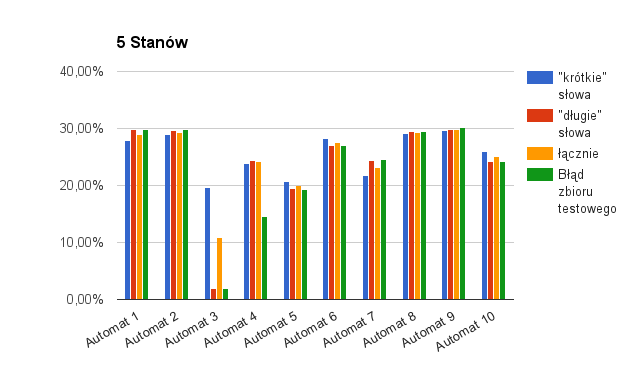
\includegraphics[width=\textwidth]{A5}
\end{figure}


\begin{table}[]
\centering 
\caption{Rekonstrukcja automatu 8-stanowego}  
\begin{tabular}{| c | c | c | c |} 
\hline \multicolumn{3}{| c |}{ Zbiór treningowy }  & Zbiór testowy \\
\hline Błąd ,,krótkich'' słów [\%] & Błąd ,,długich słów'' [\%] & Błąd łączny [\%] & Błąd zbioru testowego [\%] \\ [0.5ex]  
\hline 21,34 & 21,68 & 21,51 & 21,85 \\ 
\hline 21,65 & 22,10 & 21,87 & 22,03 \\ 
\hline 21,85 & 21,99 & 21,92 & 22,02 \\ 
\hline 21,92 & 22,06 & 21,99 & 21,93 \\ 
\hline 24,11 & 23,04 & 23,57 & 23,04 \\ 
\hline 22,17 & 22,14 & 22,15 & 22,02 \\ 
\hline 
\end{tabular} 
\end{table} 

\begin{figure}[]
\caption{Rekonstrukcja automatu 8-stanowego}%
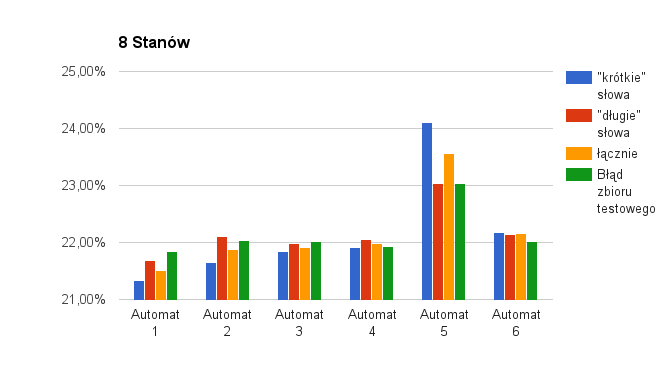
\includegraphics[width=\textwidth]{A8}
\end{figure}



\begin{table}[]
\centering 
\caption{Rekonstrukcja automatu 12-stanowego}  
\begin{tabular}{| c | c | c | c |} 
\hline \multicolumn{3}{| c |}{ Zbiór treningowy }  & Zbiór testowy \\
\hline Błąd ,,krótkich'' słów [\%] & Błąd ,,długich słów'' [\%] & Błąd łączny [\%] & Błąd zbioru testowego [\%] \\ [0.5ex]  
\hline 15,78 & 16,05 & 15,92 & 16,11 \\ 
\hline 17,31 & 17,62 & 17,46 & 17,71 \\ 
\hline 17,11 & 17,42 & 17,27 & 17,42 \\ 
\hline 17,72 & 17,46 & 17,59 & 17,64 \\ 
\hline 15,31 & 15,58 & 15,45 & 15,70 \\ 
\hline 15,58 & 15,96 & 15,77 & 15,90 \\ 
\hline 
\end{tabular} 
\end{table} 

\begin{figure}[]
\caption{Rekonstrukcja automatu 12-stanowego}%
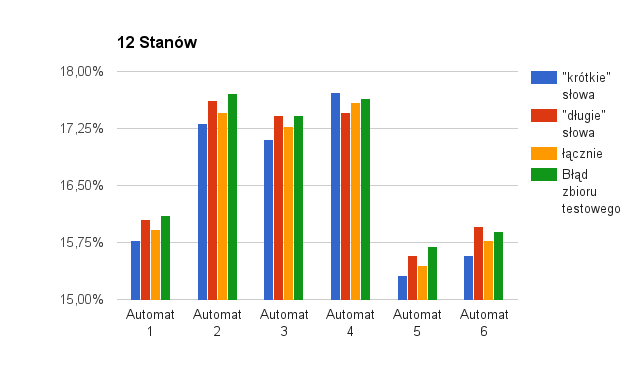
\includegraphics[width=\textwidth]{A12}
\end{figure}

\newpage

\subsection{B. Aproksymacja automatów}

%\FloatBarrier
%\newpage
\textbf{Aproksymacja automatów 20 stanowych} 

\begin{table}[] 
\centering 
\caption{Aproksymacja za pomocą automatu o 4 stanach}  
\begin{tabular}{| c | c | c | c |} 
\hline \multicolumn{3}{| c |}{ Zbiór treningowy }  & Zbiór testowy \\
\hline Błąd ,,krótkich'' słów [\%] & Błąd ,,długich słów'' [\%] & Błąd łączny [\%] & Błąd zbioru testowego [\%] \\ [0.5ex]  
\hline 27,70 & 27,93 & 27,81 & 27,86 \\ 
\hline 26,81 & 26,87 & 26,84 & 26,89 \\ 
\hline 27,42 & 27,54 & 27,48 & 27,53 \\ 
\hline 27,24 & 27,16 & 27,20 & 27,20 \\ 
\hline 27,15 & 27,00 & 27,07 & 27,00 \\ 
\hline 
\end{tabular} 
\end{table} 

\begin{figure}[]
\caption{Aproksymacja za pomocą automatu o 4 stanach}%
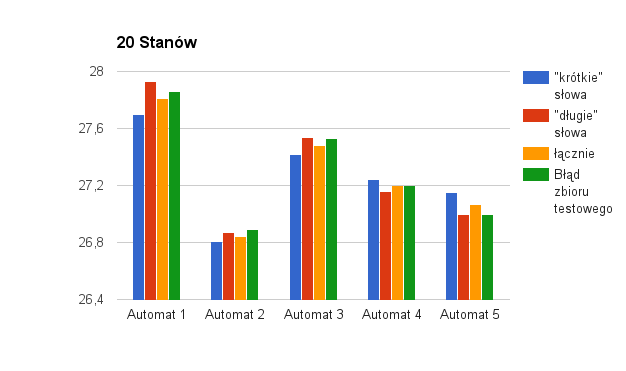
\includegraphics[width=\textwidth]{B20-4}
\end{figure}


\begin{table}[] 
\centering 
\caption{Aproksymacja za pomocą automatu o 6 stanach}  
\begin{tabular}{| c | c | c | c |} 
\hline \multicolumn{3}{| c |}{ Zbiór treningowy }  & Zbiór testowy \\
\hline Błąd ,,krótkich'' słów [\%] & Błąd ,,długich słów'' [\%] & Błąd łączny [\%] & Błąd zbioru testowego [\%] \\ [0.5ex]   
\hline 21,80 & 21,91 & 21,85 & 21,94 \\ 
\hline 20,78 & 20,54 & 20,66 & 20,73 \\ 
\hline 20,65 & 20,61 & 20,63 & 20,71 \\ 
\hline 20,93 & 20,91 & 20,92 & 21,00 \\ 
\hline 21,23 & 21,17 & 21,20 & 21,12 \\ 
\hline 
\end{tabular} 
\end{table} 

\begin{figure}[]
\caption{Aproksymacja za pomocą automatu o 6 stanach}%
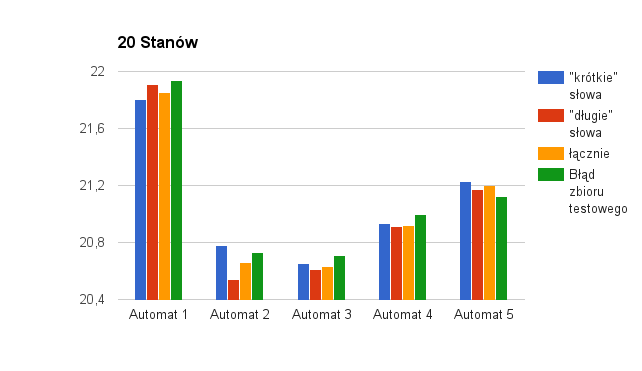
\includegraphics[width=\textwidth]{B20-6}
\end{figure}

\begin{table}[] 
\centering 
\caption{Aproksymacja za pomocą automatu o 8 stanach} 
\begin{tabular}{| c | c | c | c | } 
\hline \multicolumn{3}{| c |}{ Zbiór treningowy }  & Zbiór testowy \\
\hline Błąd ,,krótkich'' słów [\%] & Błąd ,,długich słów'' [\%] & Błąd łączny [\%] & Błąd zbioru testowego [\%] \\ [0.5ex]  
\hline 18,34 & 18,23 & 18,29 & 18,26  \\ 
\hline 18,18 & 18,44 & 18,31 & 18,42  \\ 
\hline 17,62 & 17,48 & 17,56 & 17,46  \\ 
\hline 18,73 & 18,93 & 18,83 & 18,88  \\ 
\hline 17,91 & 18,31 & 18,11 & 18,26  \\ 
\hline 
\end{tabular} 
\end{table}

\begin{figure}[]
\caption{Aproksymacja za pomocą automatu o 8 stanach}%
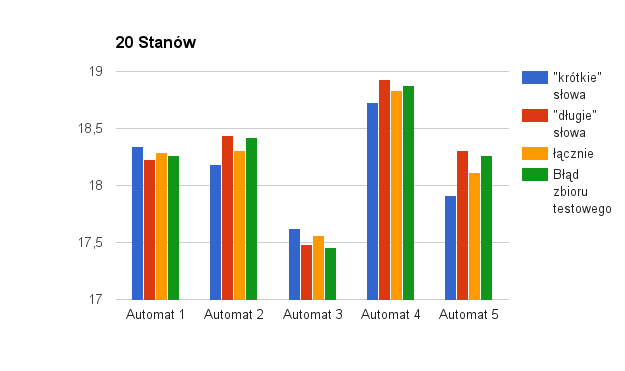
\includegraphics[width=\textwidth]{B20-8}
\end{figure}

\begin{table}[] 
\centering 
\caption{Aproksymacja za pomocą automatu o 10 stanach}  
\begin{tabular}{| c | c | c | c |} 
\hline \multicolumn{3}{| c |}{ Zbiór treningowy }  & Zbiór testowy \\
\hline Błąd ,,krótkich'' słów [\%] & Błąd ,,długich słów'' [\%] & Błąd łączny [\%] & Błąd zbioru testowego [\%] \\ [0.5ex]  
\hline 14,94 & 15,54 & 15,23 & 15,40 \\ 
\hline 14,31 & 14,54 & 14,42 & 14,53 \\ 
\hline 14,62 & 14,37 & 15,50 & 14,49 \\ 
\hline 14,64 & 14,89 & 14,76 & 14,84 \\ 
\hline 14,67 & 14,70 & 14,69 & 14,84 \\ 
\hline 
\end{tabular} 
\end{table} 

\newpage

\begin{figure}[]
\caption{Aproksymacja za pomocą automatu o 10 stanach}%
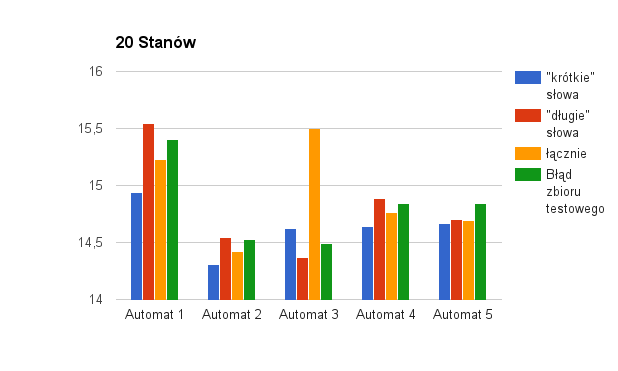
\includegraphics[width=\textwidth]{B20-10}
\end{figure}

\begin{table}[] 
\centering 
\caption{Aproksymacja za pomocą automatu o 12 stanach}  
\begin{tabular}{| c | c | c | c |} 
\hline \multicolumn{3}{| c |}{ Zbiór treningowy }  & Zbiór testowy \\
\hline Błąd ,,krótkich'' słów [\%] & Błąd ,,długich słów'' [\%] & Błąd łączny [\%] & Błąd zbioru testowego [\%] \\ [0.5ex]  
\hline 13,49 & 13,80 & 13,65 & 13,87 \\ 
\hline 13,49 & 13,63 & 13,56 & 13,57 \\ 
\hline 13,00 & 13,09 & 13,04 & 13,09 \\ 
\hline 13,11 & 13,33 & 13,22 & 13,29 \\ 
\hline 13,40 & 13,69 & 13,54 & 13,66 \\ 
\hline 
\end{tabular} 
\end{table} 

\begin{figure}[]
\caption{Aproksymacja za pomocą automatu o 12 stanach}%
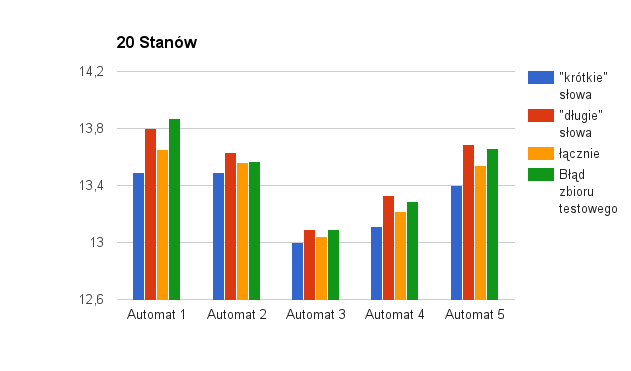
\includegraphics[width=\textwidth]{B20-12}
\end{figure}

%\FloatBarrier
\newpage
\textbf{Aproksymacja automatów 30 stanowych}

\begin{table}[] 
\centering 
\caption{Aproksymacja za pomocą automatu o 4 stanach}  
\begin{tabular}{| c | c | c | c |} 
\hline \multicolumn{3}{| c |}{ Zbiór treningowy }  & Zbiór testowy \\
\hline Błąd ,,krótkich'' słów [\%] & Błąd ,,długich słów'' [\%] & Błąd łączny [\%] & Błąd zbioru testowego [\%] \\ [0.5ex]  
\hline 26,37 & 26,54 & 26,50 & 26,77 \\ 
\hline 26,28 & 26,32 & 26,30 & 26,31 \\ 
\hline 26,32 & 26,61 & 26,46 & 26,72 \\ 
\hline 26,30 & 26,39 & 26,35 & 26,55 \\ 
\hline 26,41 & 26,40 & 26,40 & 26,49 \\ 
\hline 
\end{tabular} 
\end{table} 

\begin{figure}[]
\caption{Aproksymacja za pomocą automatu o 4 stanach}%
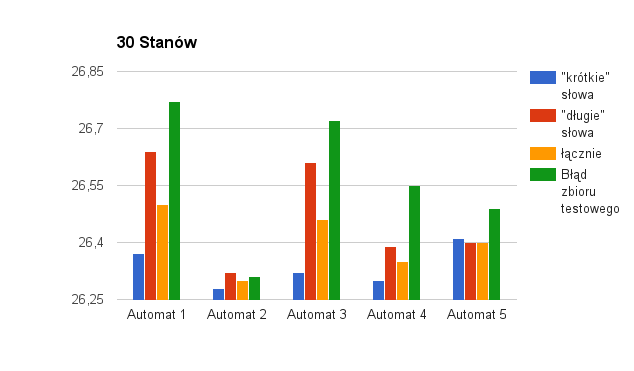
\includegraphics[width=\textwidth]{B30-4}
\end{figure}

\begin{table}[] 
\centering 
\caption{Aproksymacja za pomocą automatu o 6 stanach}  
\begin{tabular}{| c | c | c | c |} 
\hline \multicolumn{3}{| c |}{ Zbiór treningowy }  & Zbiór testowy \\
\hline Błąd ,,krótkich'' słów [\%] & Błąd ,,długich słów'' [\%] & Błąd łączny [\%] & Błąd zbioru testowego [\%] \\ [0.5ex]    
\hline 19,01 & 19,34 & 19,17 & 19,37 \\ 
\hline 19,55 & 19,57 & 19,56 & 19,49 \\ 
\hline 19,28 & 19,48 & 19,38 & 19,56 \\ 
\hline 18,89 & 19,03 & 18,96 & 19,14 \\ 
\hline 19,18 & 19,24 & 19,21 & 19,34 \\ 
\hline 
\end{tabular} 
\end{table} 

\begin{figure}[]
\caption{Aproksymacja za pomocą automatu o 6 stanach}%
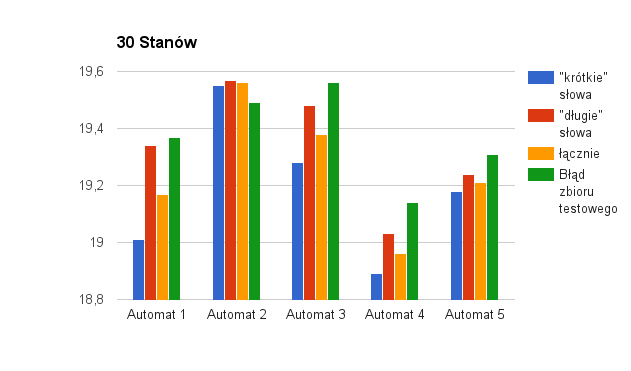
\includegraphics[width=\textwidth]{B30-6}
\end{figure}

\clearpage

\begin{table}[] 
\centering 
\caption{Aproksymacja za pomocą automatu o 8 stanach} 
\begin{tabular}{| c | c | c | c | } 
\hline \multicolumn{3}{| c |}{ Zbiór treningowy }  & Zbiór testowy \\
\hline Błąd ,,krótkich'' słów [\%] & Błąd ,,długich słów'' [\%] & Błąd łączny [\%] & Błąd zbioru testowego [\%] \\ [0.5ex]   
\hline 15,61 & 15,69 & 15,65 & 15,66  \\ 
\hline 15,75 & 15,50 & 15,63 & 15,43  \\ 
\hline 15,43 & 15,70 & 15,56 & 15,71  \\ 
\hline 15,84 & 15,97 & 15,91 & 15,95  \\ 
\hline 15,44 & 15,84 & 15,64 & 15,83  \\ 
\hline 
\end{tabular} 
\end{table}

\begin{figure}[]
\caption{Aproksymacja za pomocą automatu o 8 stanach}%
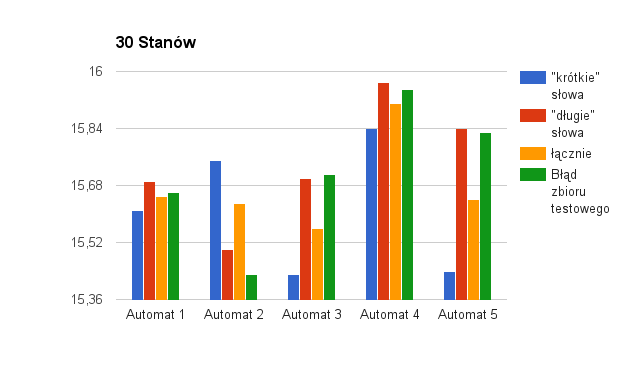
\includegraphics[width=\textwidth]{B30-8}
\end{figure}

\begin{table}[] 
\centering 
\caption{Aproksymacja za pomocą automatu o 10 stanach}  
\begin{tabular}{| c | c | c | c |} 
\hline \multicolumn{3}{| c |}{ Zbiór treningowy }  & Zbiór testowy \\
\hline Błąd ,,krótkich'' słów [\%] & Błąd ,,długich słów'' [\%] & Błąd łączny [\%] & Błąd zbioru testowego [\%] \\ [0.5ex]  
\hline 13,26 & 13,41 & 13,33 & 13,56 \\ 
\hline 13,43 & 13,35 & 13,39 & 13,35 \\ 
\hline 13,24 & 13,39 & 13,32 & 13,47 \\ 
\hline 13,25 & 13,20 & 13,22 & 13,35 \\ 
\hline 13,21 & 13,34 & 13,28 & 13,37 \\ 
\hline 
\end{tabular} 
\end{table} 

\begin{figure}[]
\caption{Aproksymacja za pomocą automatu o 10 stanach}%
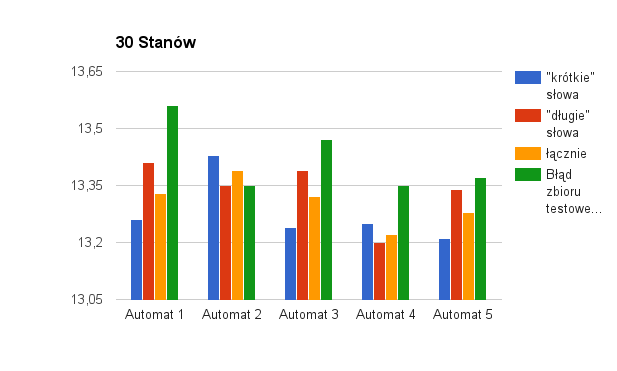
\includegraphics[width=\textwidth]{B30-10}
\end{figure}

\begin{table}[] 
\centering 
\caption{Aproksymacja za pomocą automatu o 12 stanach}  
\begin{tabular}{| c | c | c | c |} 
\hline \multicolumn{3}{| c |}{ Zbiór treningowy }  & Zbiór testowy \\
\hline Błąd ,,krótkich'' słów [\%] & Błąd ,,długich słów'' [\%] & Błąd łączny [\%] & Błąd zbioru testowego [\%] \\ [0.5ex]   
\hline 11,71 & 11,98 & 11,85 & 11,90 \\ 
\hline 11,95 & 11,65 & 11,80 & 11,70 \\ 
\hline 12,05 & 12,07 & 12,06 & 12,00 \\ 
\hline 11,75 & 12,08 & 11,92 & 12,05 \\ 
\hline 12,21 & 12,21 & 12,21 & 12,31 \\ 
\hline 
\end{tabular} 
\end{table} 

\begin{figure}[]
\caption{Aproksymacja za pomocą automatu o 12 stanach}%
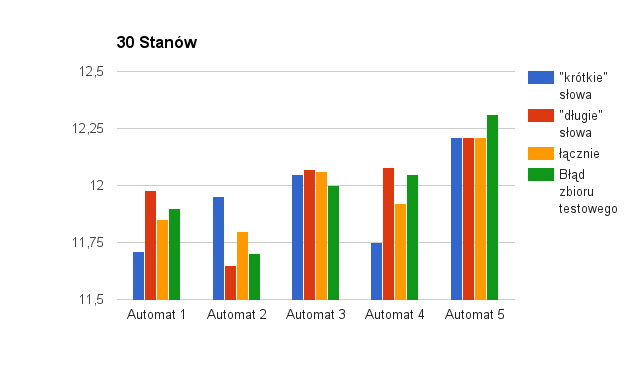
\includegraphics[width=\textwidth]{B30-12}
\end{figure}

\newpage

\textbf{Aproksymacja automatów 40 stanowych}

\begin{table}[] 
\centering 
\caption{Aproksymacja za pomocą automatu o 4 stanach}  
\begin{tabular}{| c | c | c | c |} 
\hline \multicolumn{3}{| c |}{ Zbiór treningowy }  & Zbiór testowy \\
\hline Błąd ,,krótkich'' słów [\%] & Błąd ,,długich słów'' [\%] & Błąd łączny [\%] & Błąd zbioru testowego [\%] \\ [0.5ex]  
\hline 26,52 & 26,46 & 26,49 & 26,58 \\ 
\hline 26,11 & 26,17 & 26,14 & 26,05 \\ 
\hline 26,66 & 26,85 & 26,75 & 26,74 \\ 
\hline 26,45 & 26,42 & 26,43 & 26,26 \\ 
\hline 26,58 & 26,73 & 26,65 & 26,74 \\ 
\hline 
\end{tabular} 
\end{table} 

\begin{figure}[]
\caption{Aproksymacja za pomocą automatu o 4 stanach}%
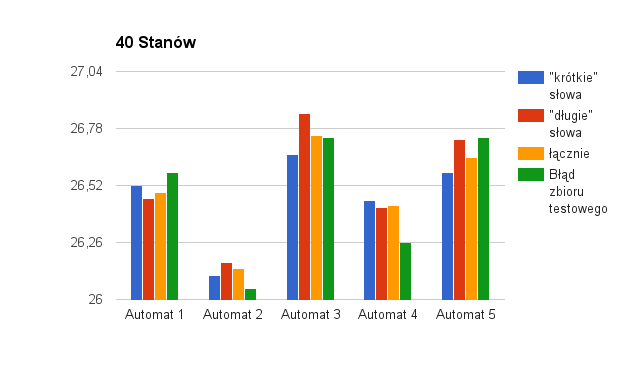
\includegraphics[width=\textwidth]{B40-4}
\end{figure}

\begin{table}[] 
\centering 
\caption{Aproksymacja za pomocą automatu o 6 stanach}  
\begin{tabular}{| c | c | c | c |} 
\hline \multicolumn{3}{| c |}{ Zbiór treningowy }  & Zbiór testowy \\
\hline Błąd ,,krótkich'' słów [\%] & Błąd ,,długich słów'' [\%] & Błąd łączny [\%] & Błąd zbioru testowego [\%] \\ [0.5ex]    
\hline 18,53 & 18,65 & 18,59 & 18,65 \\ 
\hline 18,67 & 18,39 & 18,53 & 18,47 \\ 
\hline 18,66 & 18,85 & 18,75 & 18,87 \\ 
\hline 18,61 & 18,73 & 18,67 & 18,81 \\ 
\hline 18,59 & 18,80 & 18,69 & 18,82 \\ 
\hline 
\end{tabular} 
\end{table} 

\begin{figure}[]
\caption{Aproksymacja za pomocą automatu o 6 stanach}%
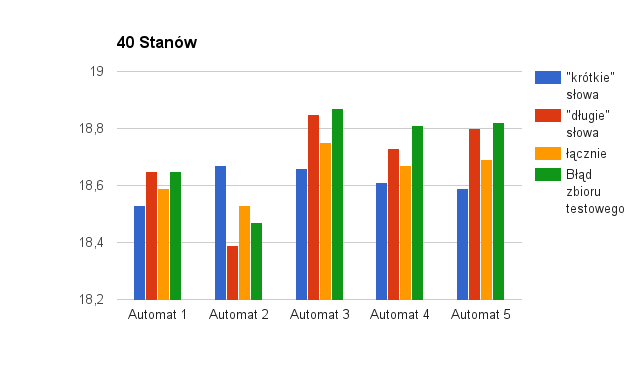
\includegraphics[width=\textwidth]{B40-6}
\end{figure}

\begin{table}[] 
\centering 
\caption{Aproksymacja za pomocą automatu o 8 stanach} 
\begin{tabular}{| c | c | c | c | } 
\hline \multicolumn{3}{| c |}{ Zbiór treningowy }  & Zbiór testowy \\
\hline Błąd ,,krótkich'' słów [\%] & Błąd ,,długich słów'' [\%] & Błąd łączny [\%] & Błąd zbioru testowego [\%] \\ [0.5ex]  
\hline 14,76 & 14,88 & 14,82 & 14,96  \\ 
\hline 14,56 & 14,71 & 14,63 & 14,59  \\ 
\hline 14,68 & 14,67 & 14,67 & 14,78  \\ 
\hline 15,22 & 15,05 & 15,13 & 18,18  \\ 
\hline 14,80 & 14,84 & 14,82 & 18,86  \\ 
\hline 
\end{tabular} 
\end{table}

\begin{figure}[]
\caption{Aproksymacja za pomocą automatu o 8 stanach}%
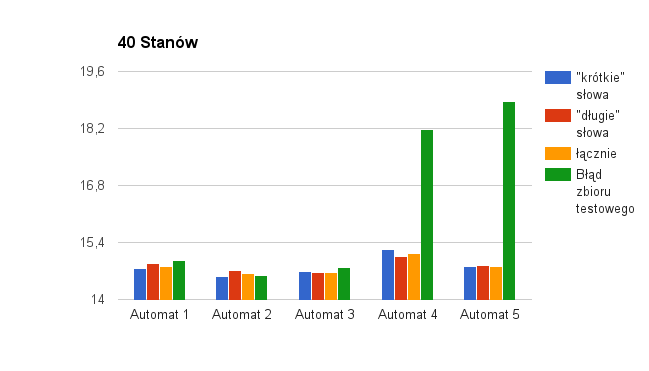
\includegraphics[width=\textwidth]{B40-8}
\end{figure}

\begin{table}[] 
\centering 
\caption{Aproksymacja za pomocą automatu o 10 stanach}  
\begin{tabular}{| c | c | c | c |} 
\hline \multicolumn{3}{| c |}{ Zbiór treningowy }  & Zbiór testowy \\
\hline Błąd ,,krótkich'' słów [\%] & Błąd ,,długich słów'' [\%] & Błąd łączny [\%] & Błąd zbioru testowego [\%] \\ [0.5ex]    
\hline 12,34 & 12,47 & 12,40 & 12,61 \\ 
\hline 12,79 & 12,88 & 12,84 & 12,97 \\ 
\hline 12,48 & 12,48 & 12,48 & 12,53 \\ 
\hline 12,83 & 12,68 & 12,70 & 12,69 \\ 
\hline 12,52 & 12,71 & 12,62 & 12,70 \\ 
\hline 
\end{tabular} 
\end{table} 

\begin{figure}[]
\caption{Aproksymacja za pomocą automatu o 10 stanach}%
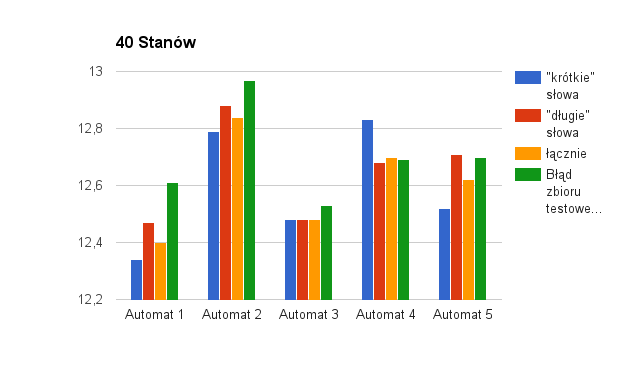
\includegraphics[width=\textwidth]{B40-10}
\end{figure}


\begin{table}[] 
\centering 
\caption{Aproksymacja za pomocą automatu o 12 stanach}  
\begin{tabular}{| c | c | c | c |} 
\hline \multicolumn{3}{| c |}{ Zbiór treningowy }  & Zbiór testowy \\
\hline Błąd ,,krótkich'' słów [\%] & Błąd ,,długich słów'' [\%] & Błąd łączny [\%] & Błąd zbioru testowego [\%] \\ [0.5ex]  
\hline 11,13 & 11,43 & 11,28 & 11,28 \\ 
\hline 11,10 & 10,98 & 11,04 & 11,02 \\ 
\hline 10,85 & 10,88 & 10,87 & 10,98 \\ 
\hline 11,00 & 11,00 & 11,00 & 11,11 \\ 
\hline 11,32 & 11,26 & 11,29 & 11,27 \\ 
\hline 
\end{tabular} 
\end{table} 

\begin{figure}[]
\caption{Aproksymacja za pomocą automatu o 12 stanach}%
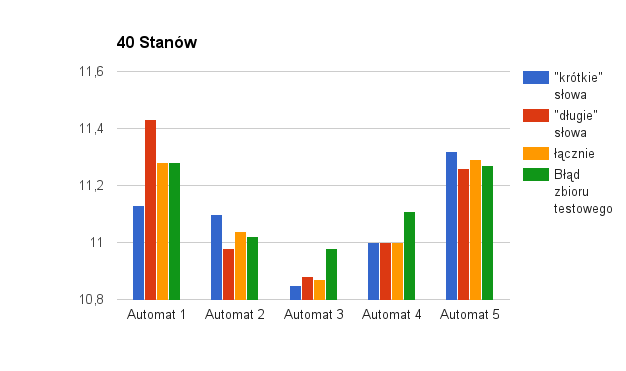
\includegraphics[width=\textwidth]{B40-12}
\end{figure}

\end{document}
